% Section 6.9: Science Data Quality Analysis (SDQA) Subsystem

\subsection{\label{sdqasubsection}Science Data Quality Analysis (SDQA) Subsystem}

Understanding the scientific quality of the data that comes out of the
processing pipelines is acutely challenging for LSST due to its
extremely large data production rate.  Traditional, human-driven
assessment techniques are simply not scalable; rather, we will require
a highly automated process for assessing quality that can be managed by
a few people.  Science Data Quality Analysis (SDQA) subsystem aims to
enable that process; that is, it is a comprehensive system
(including both automated and human-intensive components) which
collects, analyzes and records information about the quality of raw
and derived science data and makes that information to both LSST
system operators and end science users.  In practice, it will collect
summary measurements from the data pipelines and compile them into
concise reports for review by a responsible scientist.  Further, it
collate these measurements into concise metrics that compared against
benchmark values to identify problems that affect the scientific
integrity of the data products and alert the appropriate technicians.  

Initial design for SDQA was carried out prior to DC3a, but DC3a saw
the first implementation of the major components.  The subsections
that follow detail our objectives for DC3a and gauge our progress in
terms of these objectives.\footnote{Much of the design was also
  presented at the 2008 ADASS conference held at Quebec City
  \citep{laher08}}


\subsubsection{Objectives}

   The objectives for development of the SDQA subsystem in DC3a are as follows:

\begin{enumerate} 
\item{Develop a UML model for SDQA and integrate it into the overall LSST UML model.} 
\item{Develop a scheme for naming SDQA metrics. }
\item{Design and implement a first version of the database schema for SDQA.}
\item{Develop and test C++/Python code for SDQA data-container classes.}
\item{Develop and test a formatter C++ class for persisting SDQA data.}
\item{Integrate into LSST image-processing pipelines code that creates SDQA objects
for one or more SDQA metrics and persists the associated SDQA data.}
\end{enumerate}

\subsubsection{Accomplishments vs. Objectives}

Significant progress was made on Objective \#1.  SDQA domain model, use cases, 
and robustness diagrams were created and refined in LSST's Enterprise Architect 
software.  Work was done to integrate SDQA UML elements into the overall LSST
UML model.  Defined were the following basic SDQA objects:

\begin{description}
\item{\it SDQA Metric.}
These are diverse, predefined measures that characterize image-data quality; 
e.g., image statistics, astrometric and photometric figures of merit and associated 
errors, counts of various things, like extracted sources, etc.  Attributes of the
SDQA Metric class include name, physical units, and definition.  
\item{\it SDQA Rating.}
An SDQA Rating is 
the computed or derived value of an SDQA Metric and its uncertainty for a specific
image or image data set.  
\item{\it SDQA Threshold.}
An SDQA Threshold defines for a given SDQA Metric the 
upper and lower limits of SDQA-Rating values that indicate acceptable image-data 
quality.  \item{\it SDQA Image Status.}
An SDQA Image Status is the overall quality tag assigned to an image
after processing by the automated SDQA subsystem embedded in the image-processing
pipeline; attributes of SDQA Image Status include descriptive moniker and definition.
\end{description}

Objective \#2 was accomplished to the extent that is possible this early in the 
project.  The results of this substantial effort were written up on a Trac 
page\footnote{http://lsstdev.ncsa.uiuc.edu/trac/wiki/MetricsForSDQA}, which has 
enabled a wide-audience open discussion of the SDQA Metrics under consideration.
Additional metrics will be defined for DC3b that are informed by quantities of interest 
gleaned from our experience with the DC3a pipeline processing.

We designed and implemented a first version of the database schema for SDQA in fulfillment
of Objective \#3.  Figure~\ref{DB} shows the portion of our SDQA database-schema design
that associates SDQA Ratings with amplifier-level images.  
The primary advantage of this schema design is that persisting additional SDQA Metrics
does not require a schema change; instead you simply add new records to the SDQA\_Metric
and SDQA\_Threshold database tables to define the new SDQA Metrics and associated thresholds.
Our DC3a implementation also
includes tables for associating SDQA Ratings with image data at the CCD and FPA levels.
The schema's tables closely parallel the SDQA classes that we have identified in our UML (universal modeling language) design.

\begin{figure}[htb]
\begin{centering}
%\epsscale{0.5}
%\plotone{images/O7A2_1}
%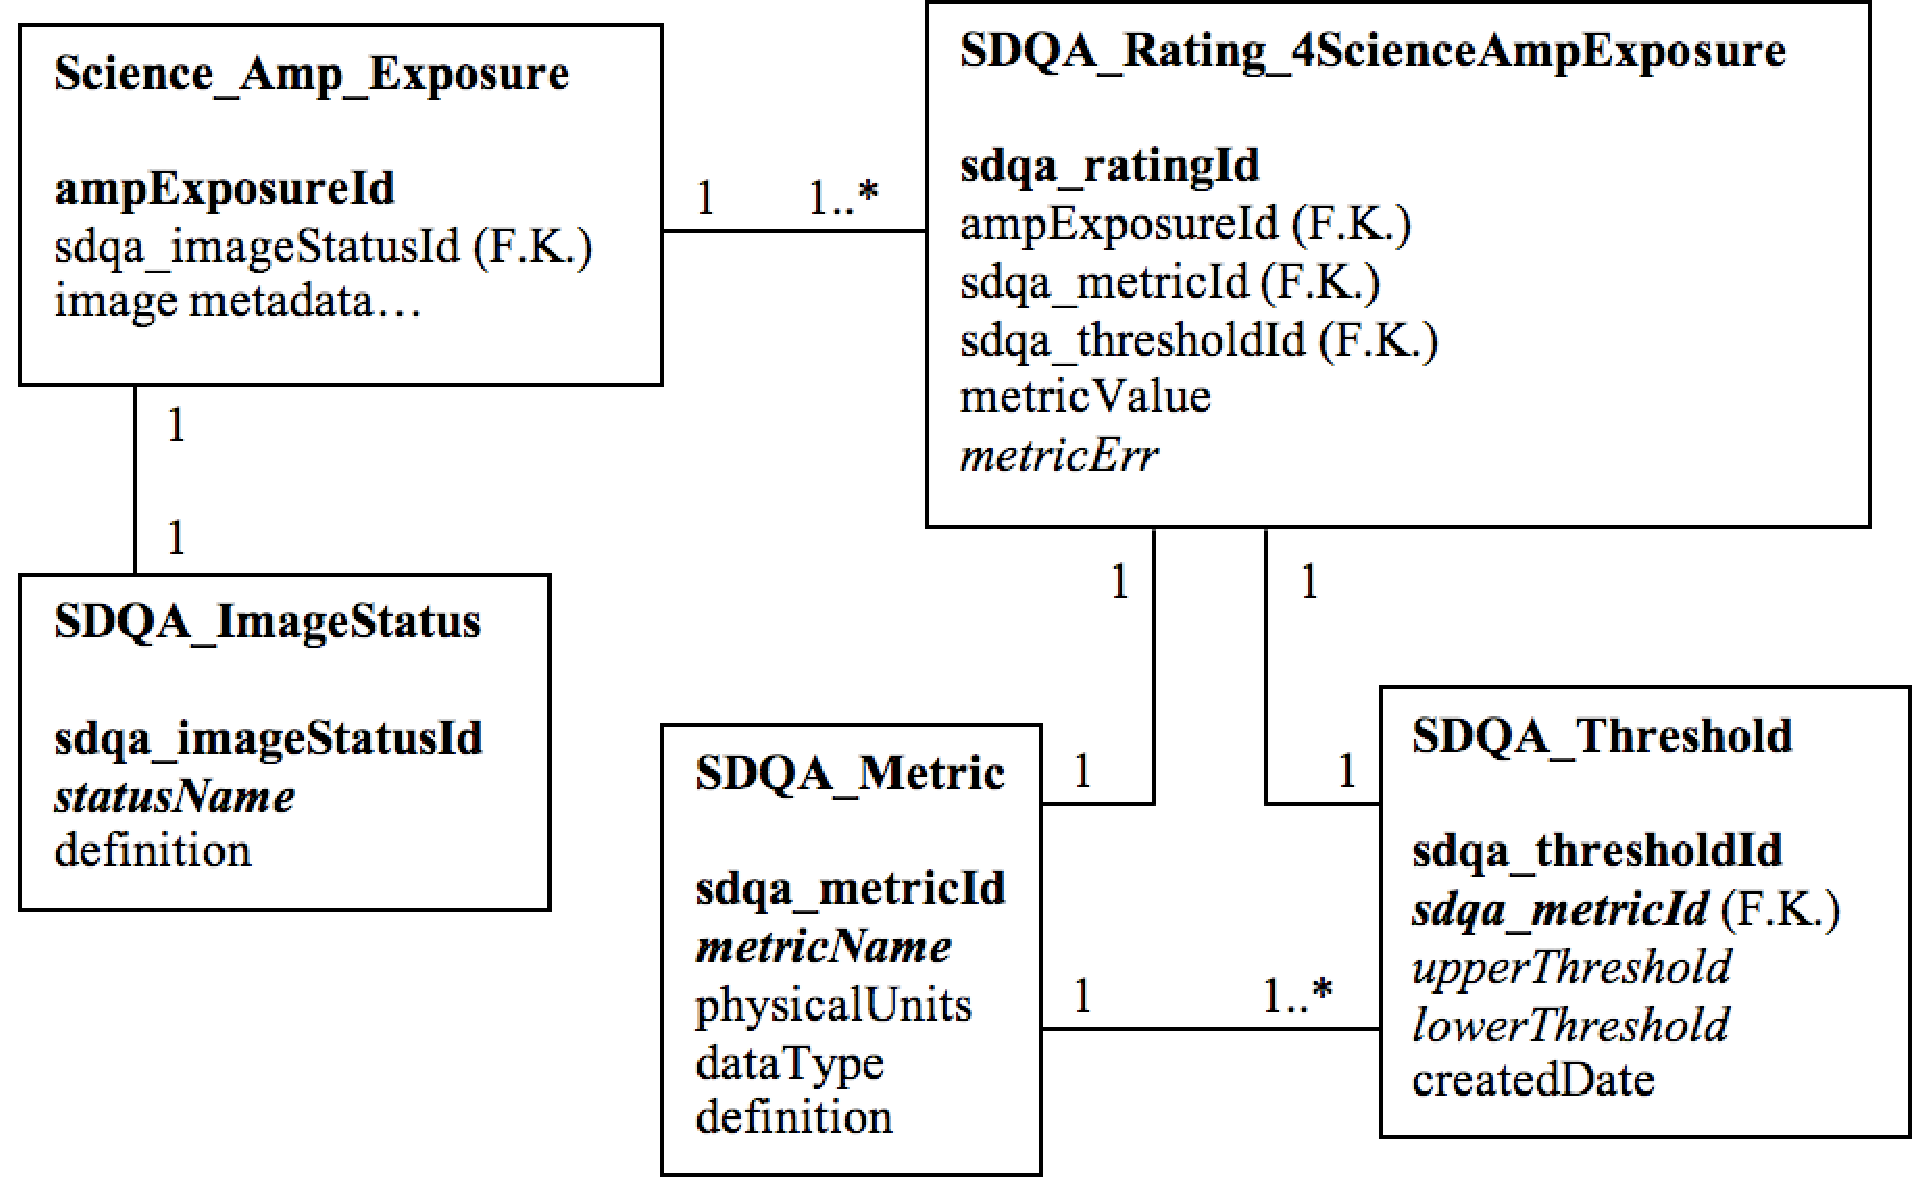
\includegraphics[scale=0.5,bb=0 0 925 573]{images/O7A2_1}
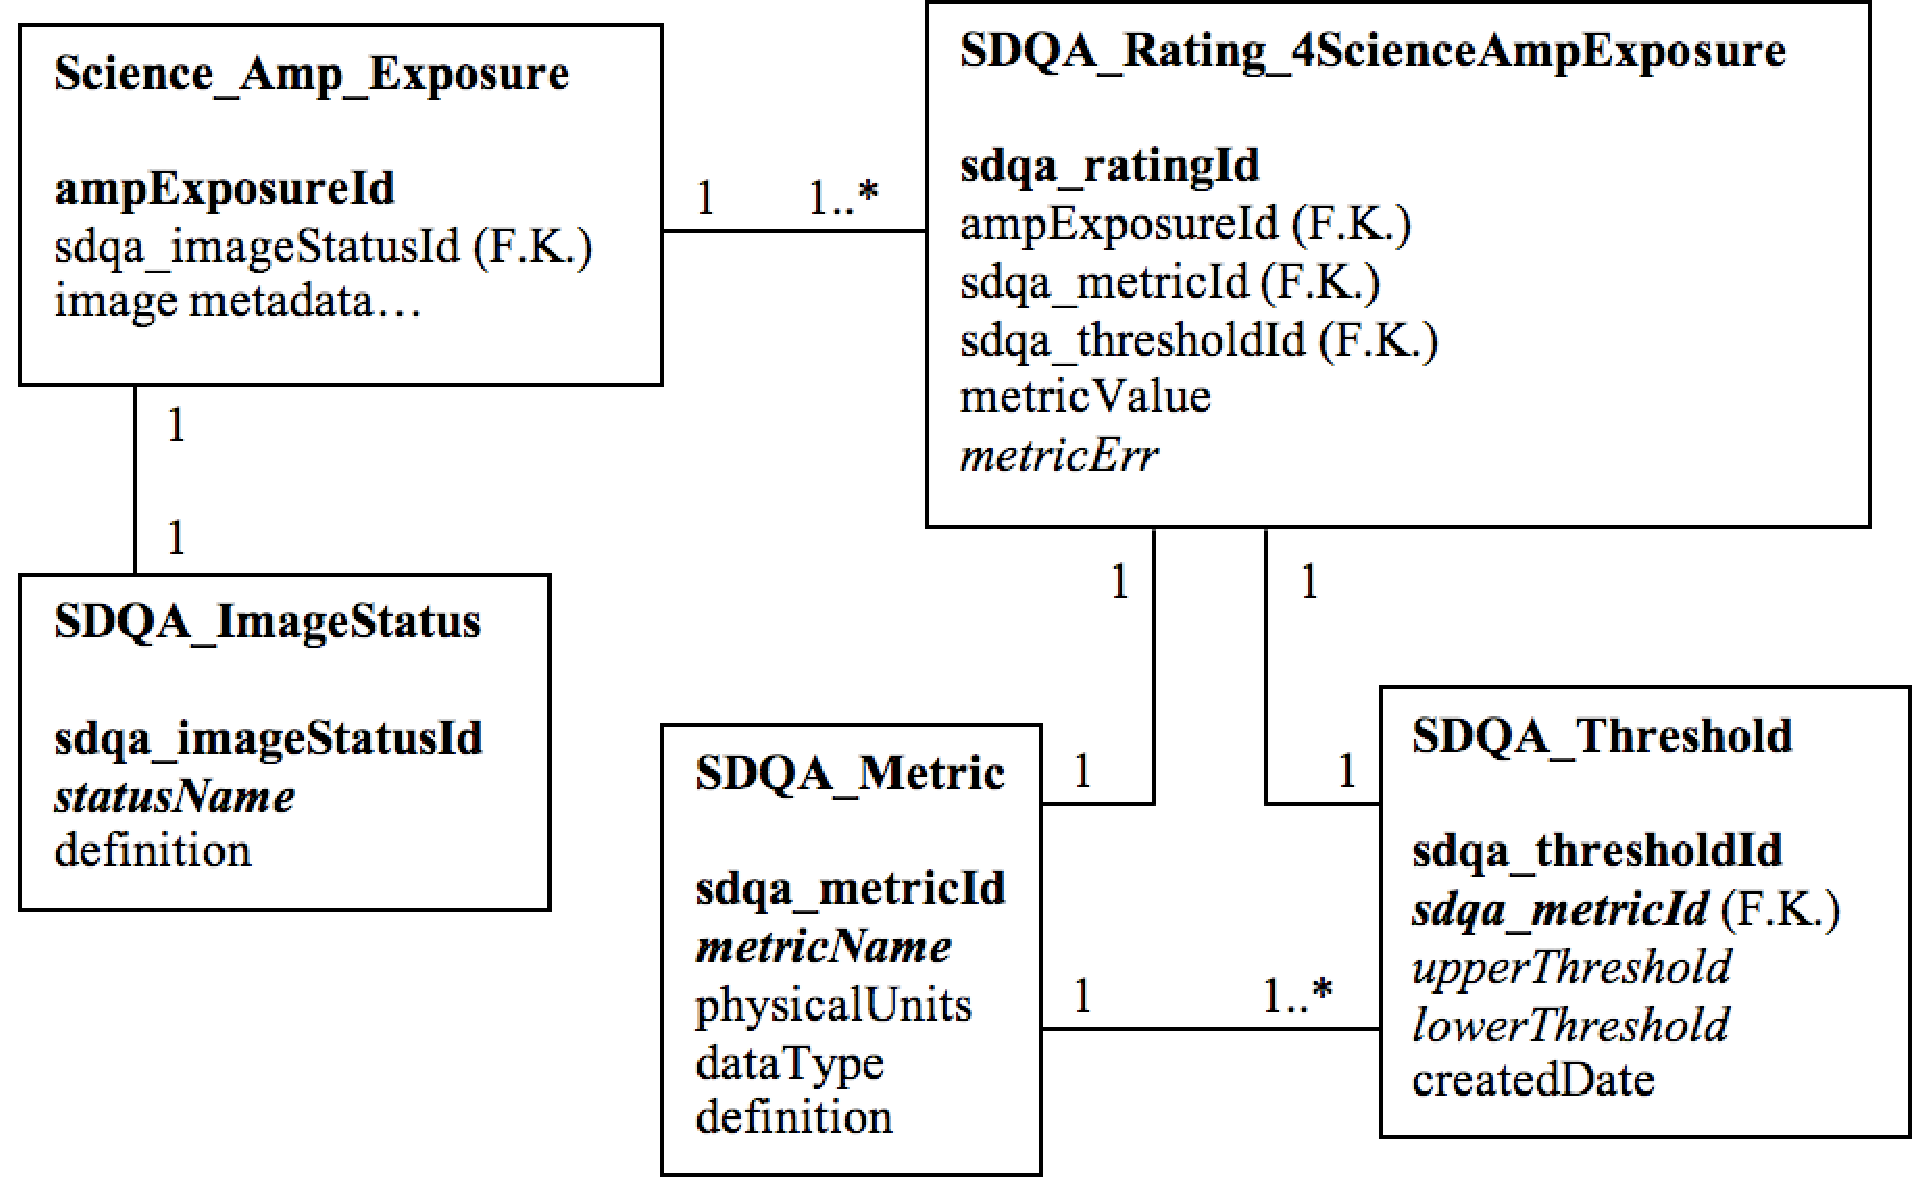
\includegraphics[scale=0.4]{images/O7A2_1}
\caption{SDQA database-schema design (``F.K.'' stands for foreign key, and ``1~{\jot 24pt}~1*..'' stands for one record to many records).} 
 \label{DB}
\end{centering}
\end{figure}

The Science\_Amp\_Exposure database table stores metadata for
processed images associated with independently read-out 
512$\times$2048-pixel portions of 
raw images (called amplifier 
segments).  The sdqa\_imageStatusId field in this table points to the grade
category determined for the image by the SDQA subsystem (although this was not populated
in DC3a, it will be done in DC3b).  
The SDQA\_Rating\_4ScienceAmpExposure database table is associated with 
the Science\_Amp\_Exposure database table in a one-to-many
relationship.  A processed image, in general, has multiple SDQA ratings, which
are computed at various pipeline stages, temporarily stored in pipeline-shared memory, and 
ultimately persisted in the database.


We accomplished Objectives \#4 and \#5 by developing and testing object-oriented C++
source code for the following classes:

\begin{itemize}
\item{SdqaMetric}
\item{SdqaRating}
\item{PersistableSdqaRatingVector}
\item{SdqaThreshold}
\item{SdqaImageStatus}
\item{SdqaRatingFormatter}
\end{itemize}

\noindent
In addition, we implemented SWIG wrappers for usage of these classes by Python scripts
directly.  We verified all SDQA-related source code by creating unit tests and assuring
their successful execution.  The unit test for the SDQA Rating Formatter involved 
persisting SDQA Ratings in a test database.  

All software coding was done carefully to assure that LSST coding guidelines were followed.

Although the SdqaRatingFormatter class has basic functionality for persisting SDQA Ratings
in DbStorage, it lacks capabilities for DbTsvStorage, BoostStorage, and XmlStorage.  This
will be remedied in DC3b, along with a few other inefficiencies pointed out by K.-T. Lim.

We created a package called ``sdqa'' in the LSST SVN repository and committed the SDQA-related source code there.  Release 3.0.3 of the sdqa package was used in the 
final testing for DC3a.

The next subsection demonstrates how Objective \#6 was met.


\subsubsection{Sample DC3a SDQA Ratings}

To accomplish our DC3a objective of persisting SDQA Ratings, the
image-processing pipelines were modified to instantiate SDQA-Rating
objects for various SDQA Metrics of interest in DC3a.  A tutorial was
written to give the application developers explicit instructions on
how to persist SDQA
Ratings\footnote{http://lsstdev.ncsa.uiuc.edu/trac/wiki/SdqaRatingTutorial}.
The following example illustrates how SDQA Ratings can be used to
assess the quality of the IPSD pipeline.   Below is a sampling of
ratings that were persisted to the database during a particular
production run (run ID {\tt rlp1188}):

{\tiny
\begin{verbatim}
+----------------------------+----------+---------------------+--------------------+---------------------+---------------------+
| metricName                 | count(*) | min(metricValue)    | max(metricValue)   | avg(metricValue)    | stddev(metricValue) |
+----------------------------+----------+---------------------+--------------------+---------------------+---------------------+
| ip.diffim.kernelSum        |      558 |  -0.657514177126991 |   7.98916588029419 |     4.7838537751288 |      1.420147681719 | 
| ip.diffim.residuals        |      558 | -0.0328804743717919 | 0.0019883894744249 | -0.0021186088057241 |  0.0037378047459525 | 
| ip.isr.numCosmicRayPixels  |      558 |                   0 |                  0 |                   0 |                   0 | 
| ip.isr.numSaturatedPixels  |      558 |                   0 |               2033 |      137.8853046595 |     381.85356427703 | 
| phot.psf.numAvailStars     |      279 |                   4 |                 25 |     12.992831541219 |     4.0789632806315 | 
| phot.psf.numGoodStars      |      279 |                   4 |                 25 |     12.931899641577 |     4.0955024257056 | 
| phot.psf.spatialFitChi2    |      279 |    5.02278757095337 |   1727.95910644531 |     118.54034705316 |     199.66763559788 | 
| phot.psf.spatialLowOrdFlag |      279 |                   0 |                  0 |                   0 |                   0 | 
+----------------------------+----------+---------------------+--------------------+---------------------+---------------------+
8 rows in set (0.01 sec)
\end{verbatim}
}

\noindent
This summary of the metrics was generated with the following SQL
database query:

{\small
\begin{verbatim}
select b.metricName, count(*), min(metricValue), max(metricValue),
       avg(metricValue), stddev(metricValue) 
from sdqa_Rating_ForScienceAmpExposure a, sdqa_Metric b 
where a. sdqa_metricId=b.sdqa_metricId 
group by b.metricName;
\end{verbatim}
}

For each amplifier-level image processed, SDQA Ratings for eight different SDQA Metrics 
were persisted in the database by the pipelines.  Four SDQA ratings were computed by
the PSF pipeline, two by the ISR pipeline, and two by the difference-imaging pipeline.
That different pipelines were able to persist SDQA Ratings demonstrates the flexibility of the design.

Although demonstrating the utility of specific SDQA ratings was not an
objective of DC3a (it will be an objective for DC3b), these numbers do
reveal something of the character of the processing.  Our DC3a results
analysis has suggested that extreme values of {\tt
  ip.diffim.kernelSum} are correlated with bad subtractions between
image and template, which are ultimately caused by bad astrometry.
Despite this, we do see that kernels are being generated with the
expected statistics; that is, {\tt ip.diffim.residuals} has a
near-zero mean (compared to its RMS).   The results for {\tt
  ip.isr.numCosmicRayPixels} show that no cosmic rays were detected
which may indicate a threshold-tuning issue.  Finally, our experience
has shown that there is a correlation between {\tt
  phot.psf.numGoodStars} and the positional uncertainties of
PSF-fitted source detections, and so it is expected that this will be 
a useful diagnostic.

The information in the above table represents the kind of information
that could be included in a nightly SDQA summary.  Since the SDQA
ratings are stored in the database, it is easy to construct a variety
of useful queries; e.g., all {\tt phot.psf.numAvailStars} values for a
given night, CCD, and filter.

Although SDQA Thresholds were not tuned for DC3a, we expect this to be
a component of the work for DC3b.


\subsubsection{Advanced Assessment Techniques}

In our ADASS paper \citet{laher08}, we pointed out that the method of 
artificial neural networks is particularly promising for classifying images in 
terms of SDQA (see Figure~\ref{ANN}).  In late 2008 we undertook some work 
involving ANNs to demonstrate that various attributes of extracted
source detections could be used to differentiate between variable QSOs
and non-variable white dwarfs \citet{borne09}.  Our completeness and
reliability results showed that ANNs  are superior to the method of
segmenting the two populations in conventional color-color plots\footnote{
http://spider.ipac.caltech.edu/staff/laher/lsst/borne\_696\_Jan09-ver2.pdf
}.

\begin{figure}[htb]
\begin{centering}
% \epsscale{0.2}
% \plotone{images/O7A2_2}
%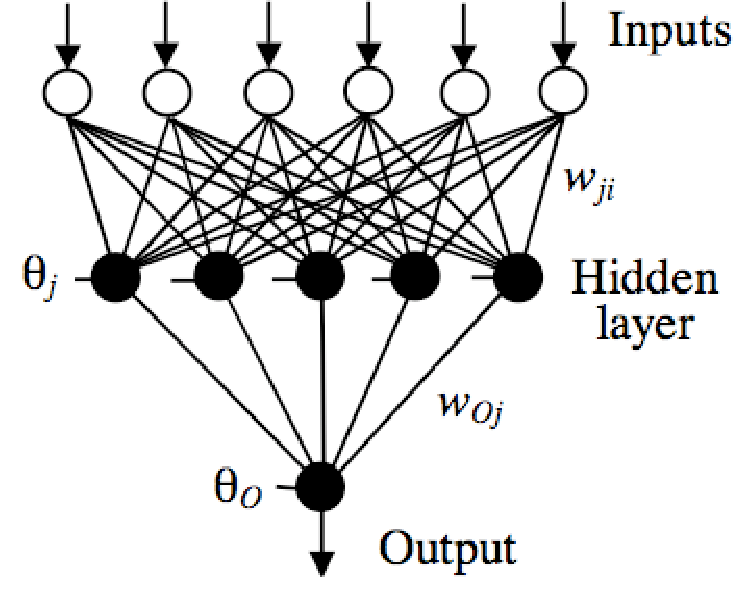
\includegraphics[scale=0.5,bb=0 0 363 285]{images/O7A2_2}
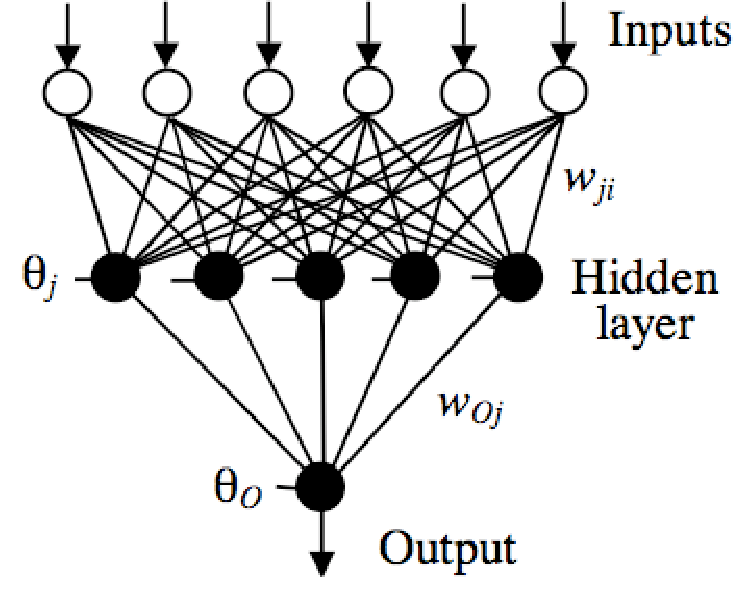
\includegraphics[width=3in]{images/O7A2_2}
\caption{Artificial neural network with single-hidden-layer architecture.} 
 \label{ANN}
\end{centering}
\end{figure}


One of IPAC's current projects is development of image-processing pipelines and data archive
for the Palomar Transient Factory (PTF), a new 12-CCD camera recently installed on the Palomar
48'' Schmidt Telescope.  This camera is now in operations and acquires up to $\approx 4,800$
CCD images per night (2K$\times$4K pixels per CCD), 
which are subsequently sent to IPAC for processing and archiving.  
While this project is separately funded, we have been able to use
it fruitfully as a test bed for prototyping LSST-SDQA-subsystem designs.  
To be clear, the utility of PTF for our LSST purposes are:

\begin{enumerate} 
\item{Validating our choices for metrics that may be useful for LSST (since PTF is a 
time-domain project with some overlapping science goals).}
\item{Technology exploration.}
\item{Exploring visualization strategies for representing very complex and 
voluminous SDQA data in a comprehendible way.}
\end{enumerate} 

We have
implemented for PTF a fully automated SDQA subsystem of the design essentially
envisioned for LSST.  The PTF image-processing pipeline now populates more than 40 different
SDQA metrics in the PTF database.  A process for thresholding SDQA ratings and determining 
SDQA statuses for processed images has been implemented as a database stored function and
integrated into the PTF image-processing pipeline.  An indispensible software tool developed 
as a result of this effort is a web-browser-based SDQA GUI, which facilitates viewing of raw and
processed images and time-series plots of SDQA ratings over a specified observing night 
(see Figures~\ref{PTFSDQAGUI1} and~\ref{PTFSDQAGUI2}).  Much of the source 
code for the PTF SDQA GUI was leveraged from Java classes developed over the last ten years at 
the Spitzer Science Center (SSC) for observation planning, image visualization, and the
Spitzer Heritage Archive interface.  The PTF SDQA GUI is a Google Web Toolkit application that
queries the PTF database for image metadata and SDQA data to display and plot.  One of our
objectives for LSST in DC3b is to further develop the SDQA GUI for LSST use, i.e., set it up to 
query and visualize LSST databases and image archives.

\begin{figure}[htbp]
\begin{centering}
% \epsscale{1.0}
% \plotone{images/PTFSDQSGUI1}
%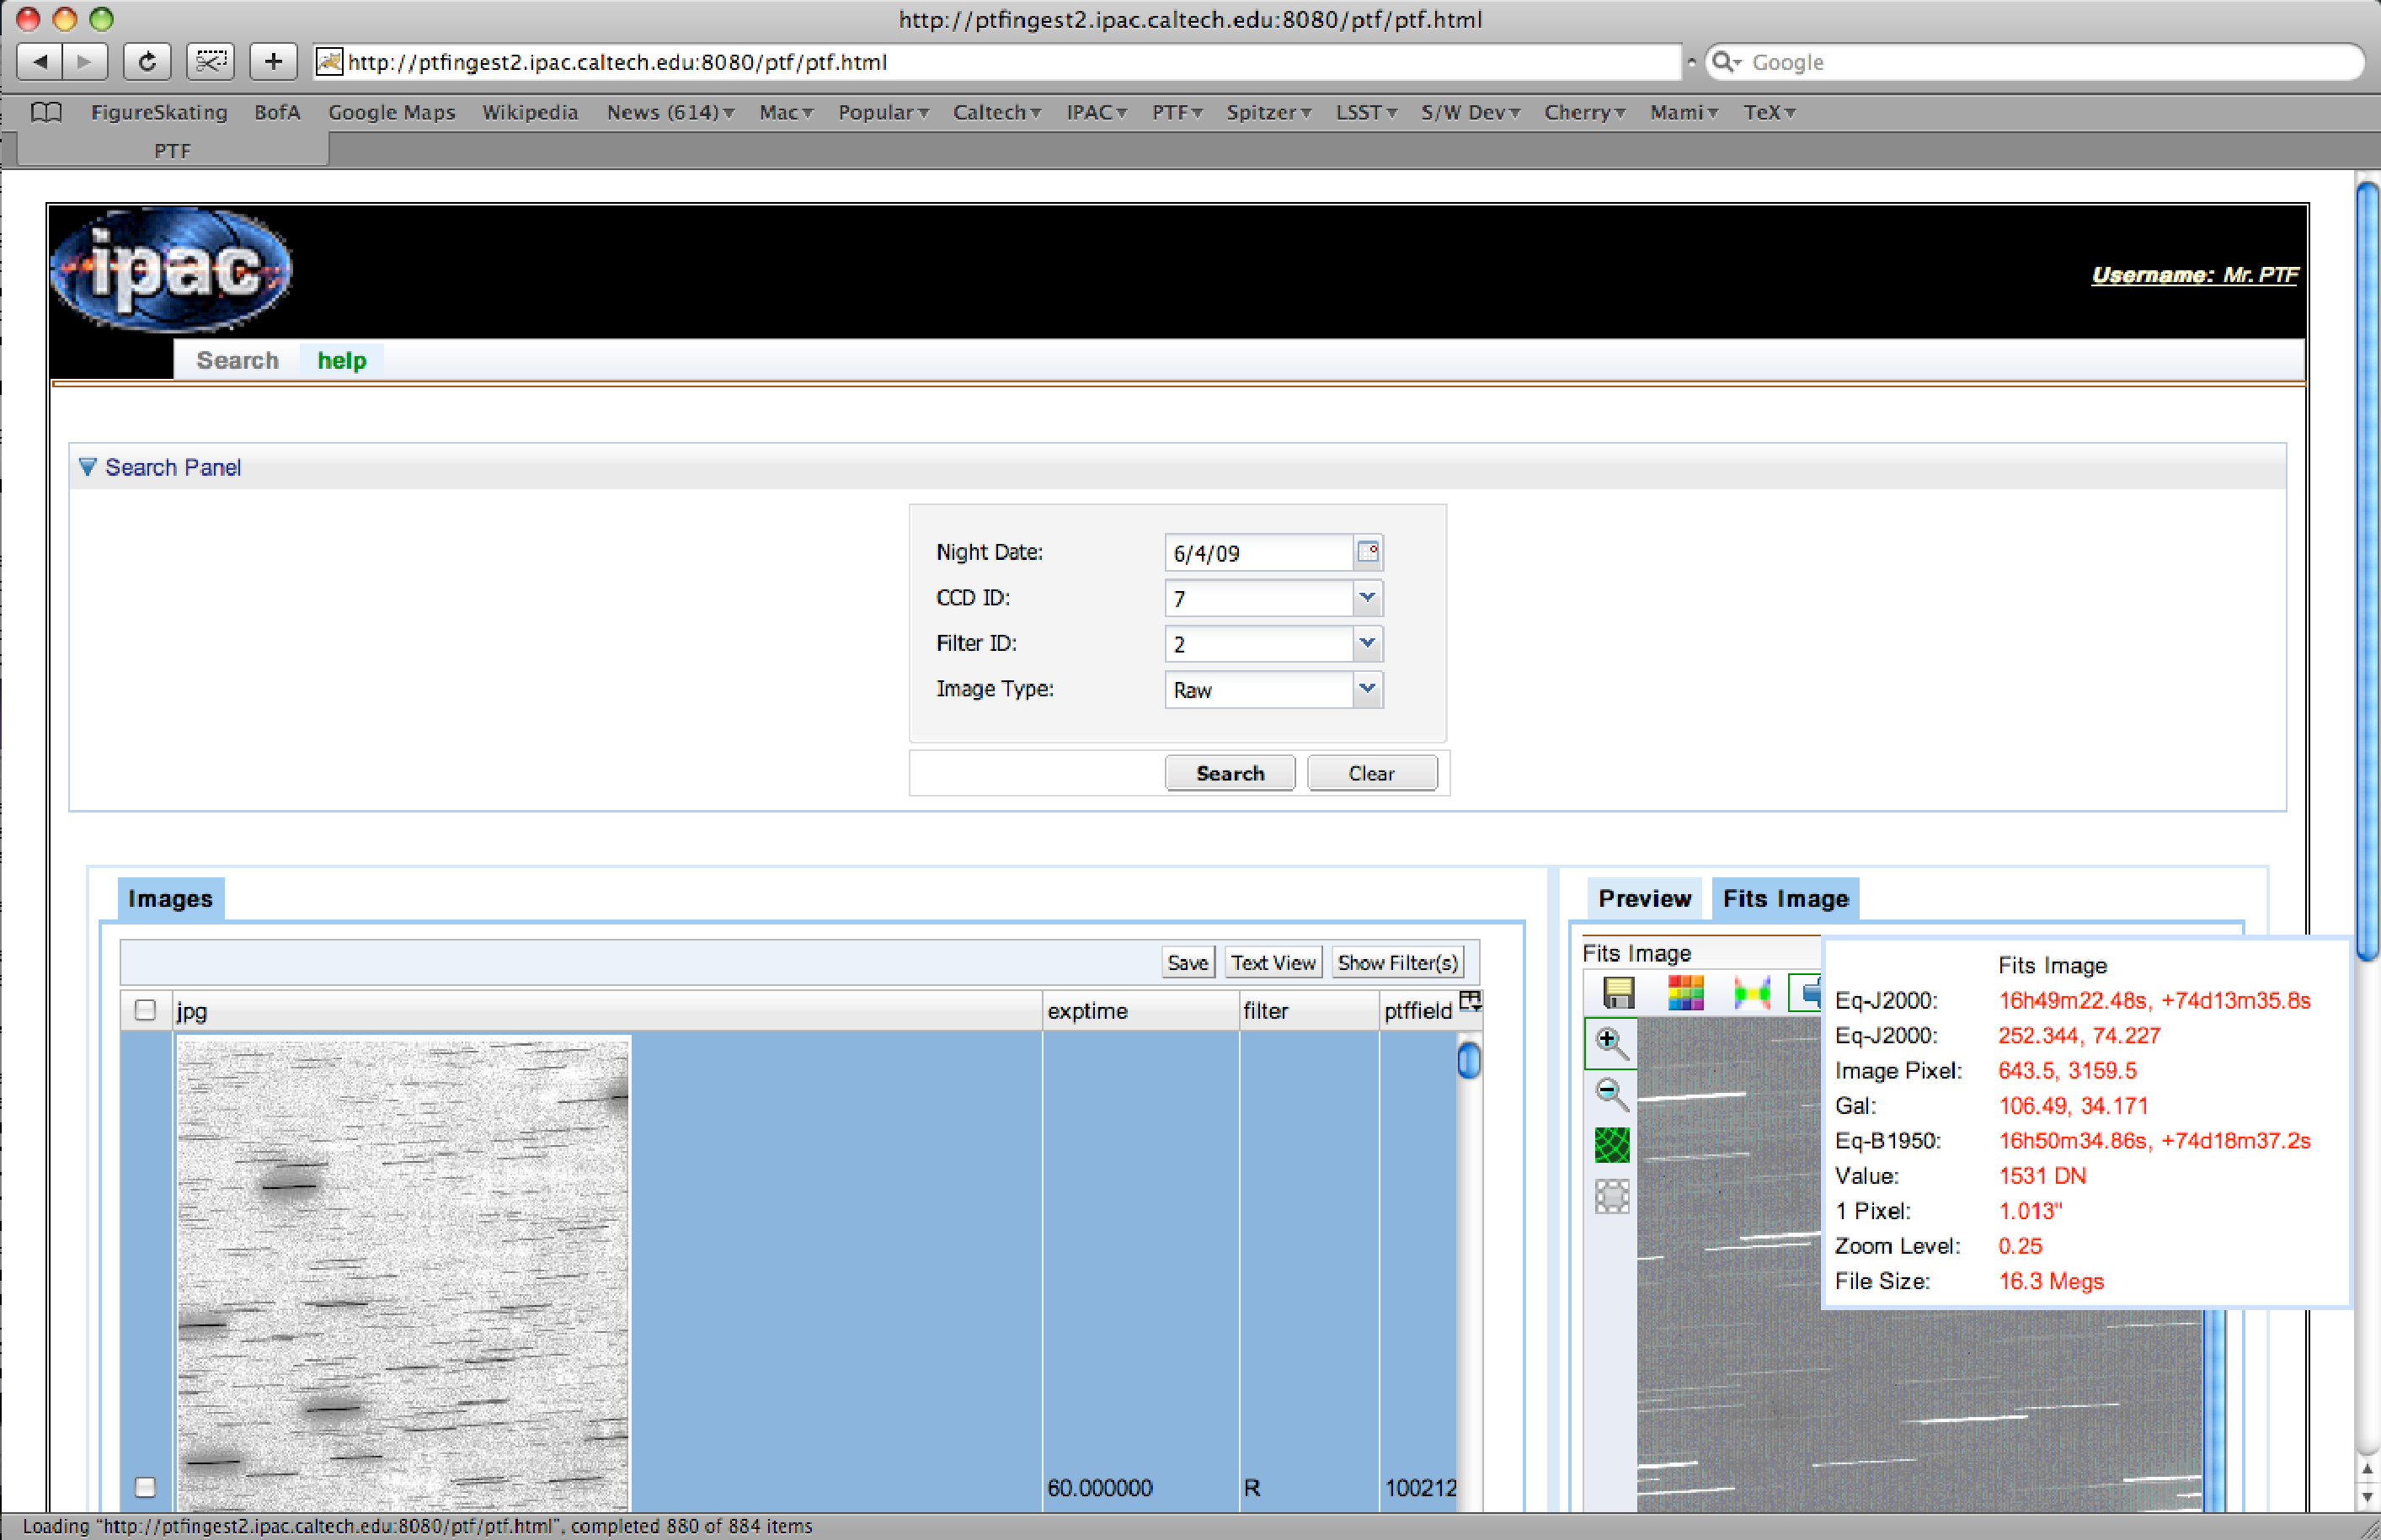
\includegraphics[width=\textwidth,scale=0.5,bb=0 0 1357 878,clip]{images/PTFSDQSGUI1}
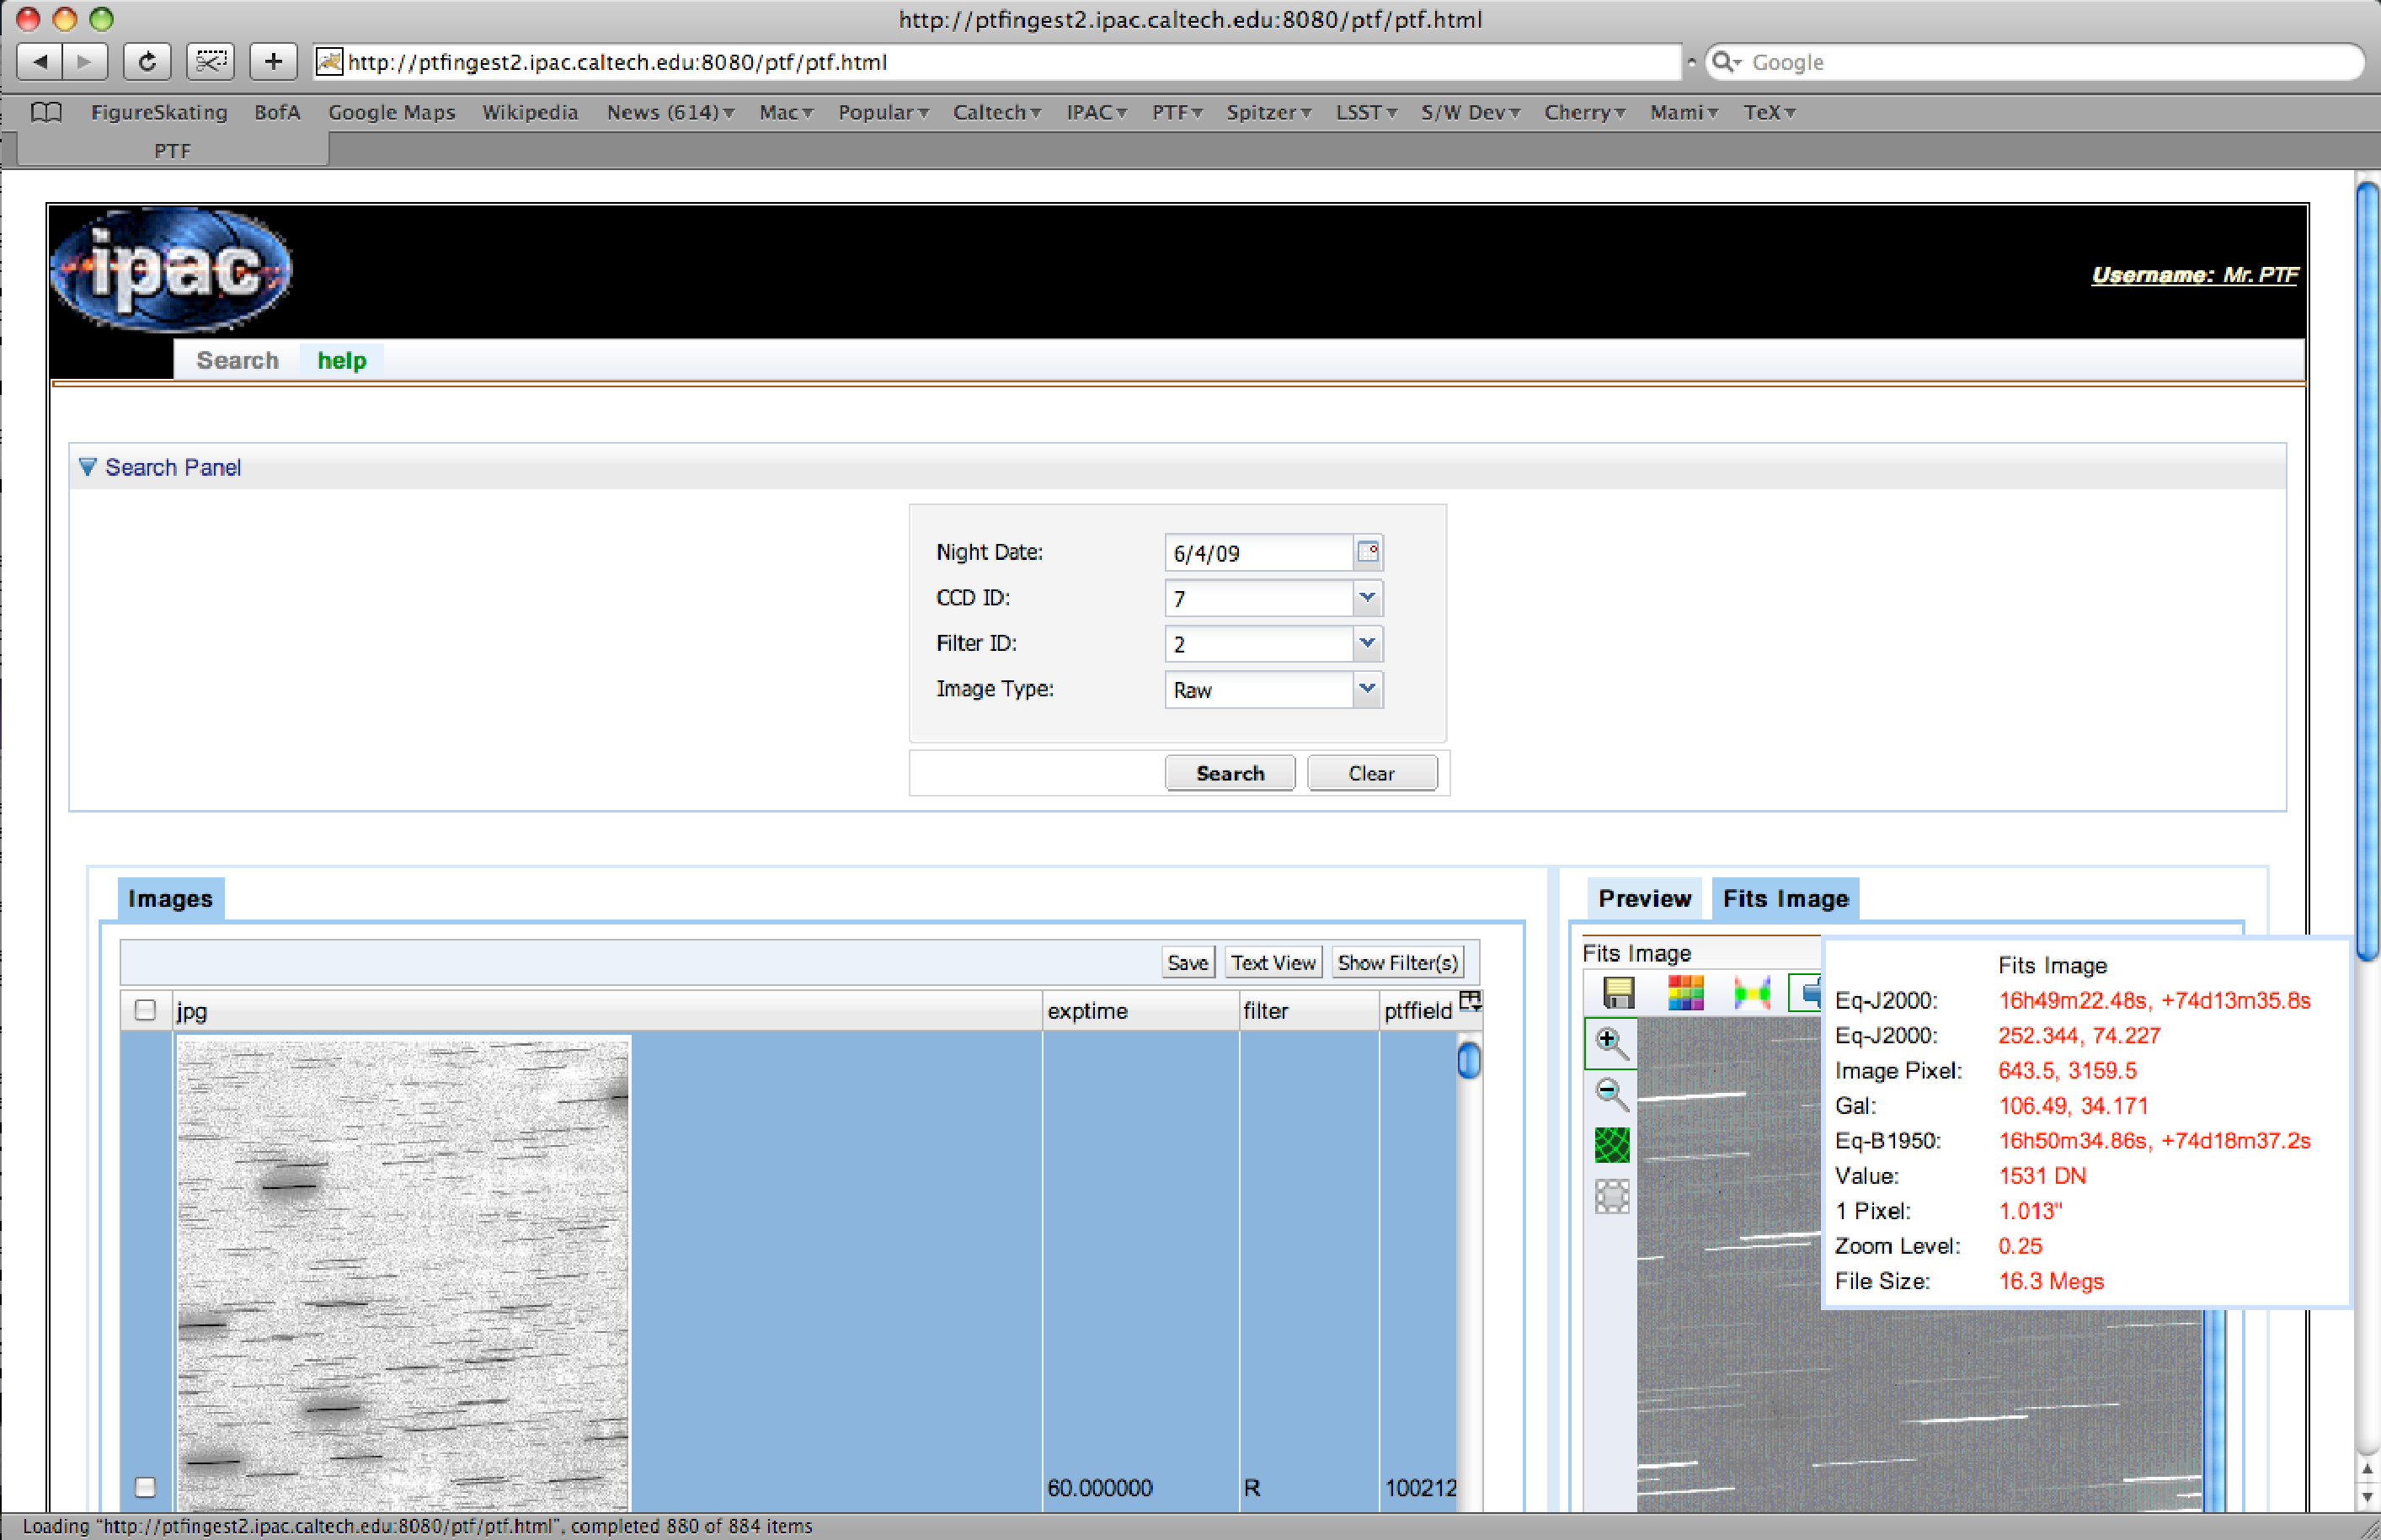
\includegraphics[width=5in]{images/PTFSDQSGUI1}
\caption{PTF SDQA GUI screen shot showing image display from query of PTF database.} 
 \label{PTFSDQAGUI1}
\end{centering}
\end{figure}

\begin{figure}[htbp]
\begin{centering}
%\epsscale{1.0}
%\plotone{images/PTFSDQSGUI2}
%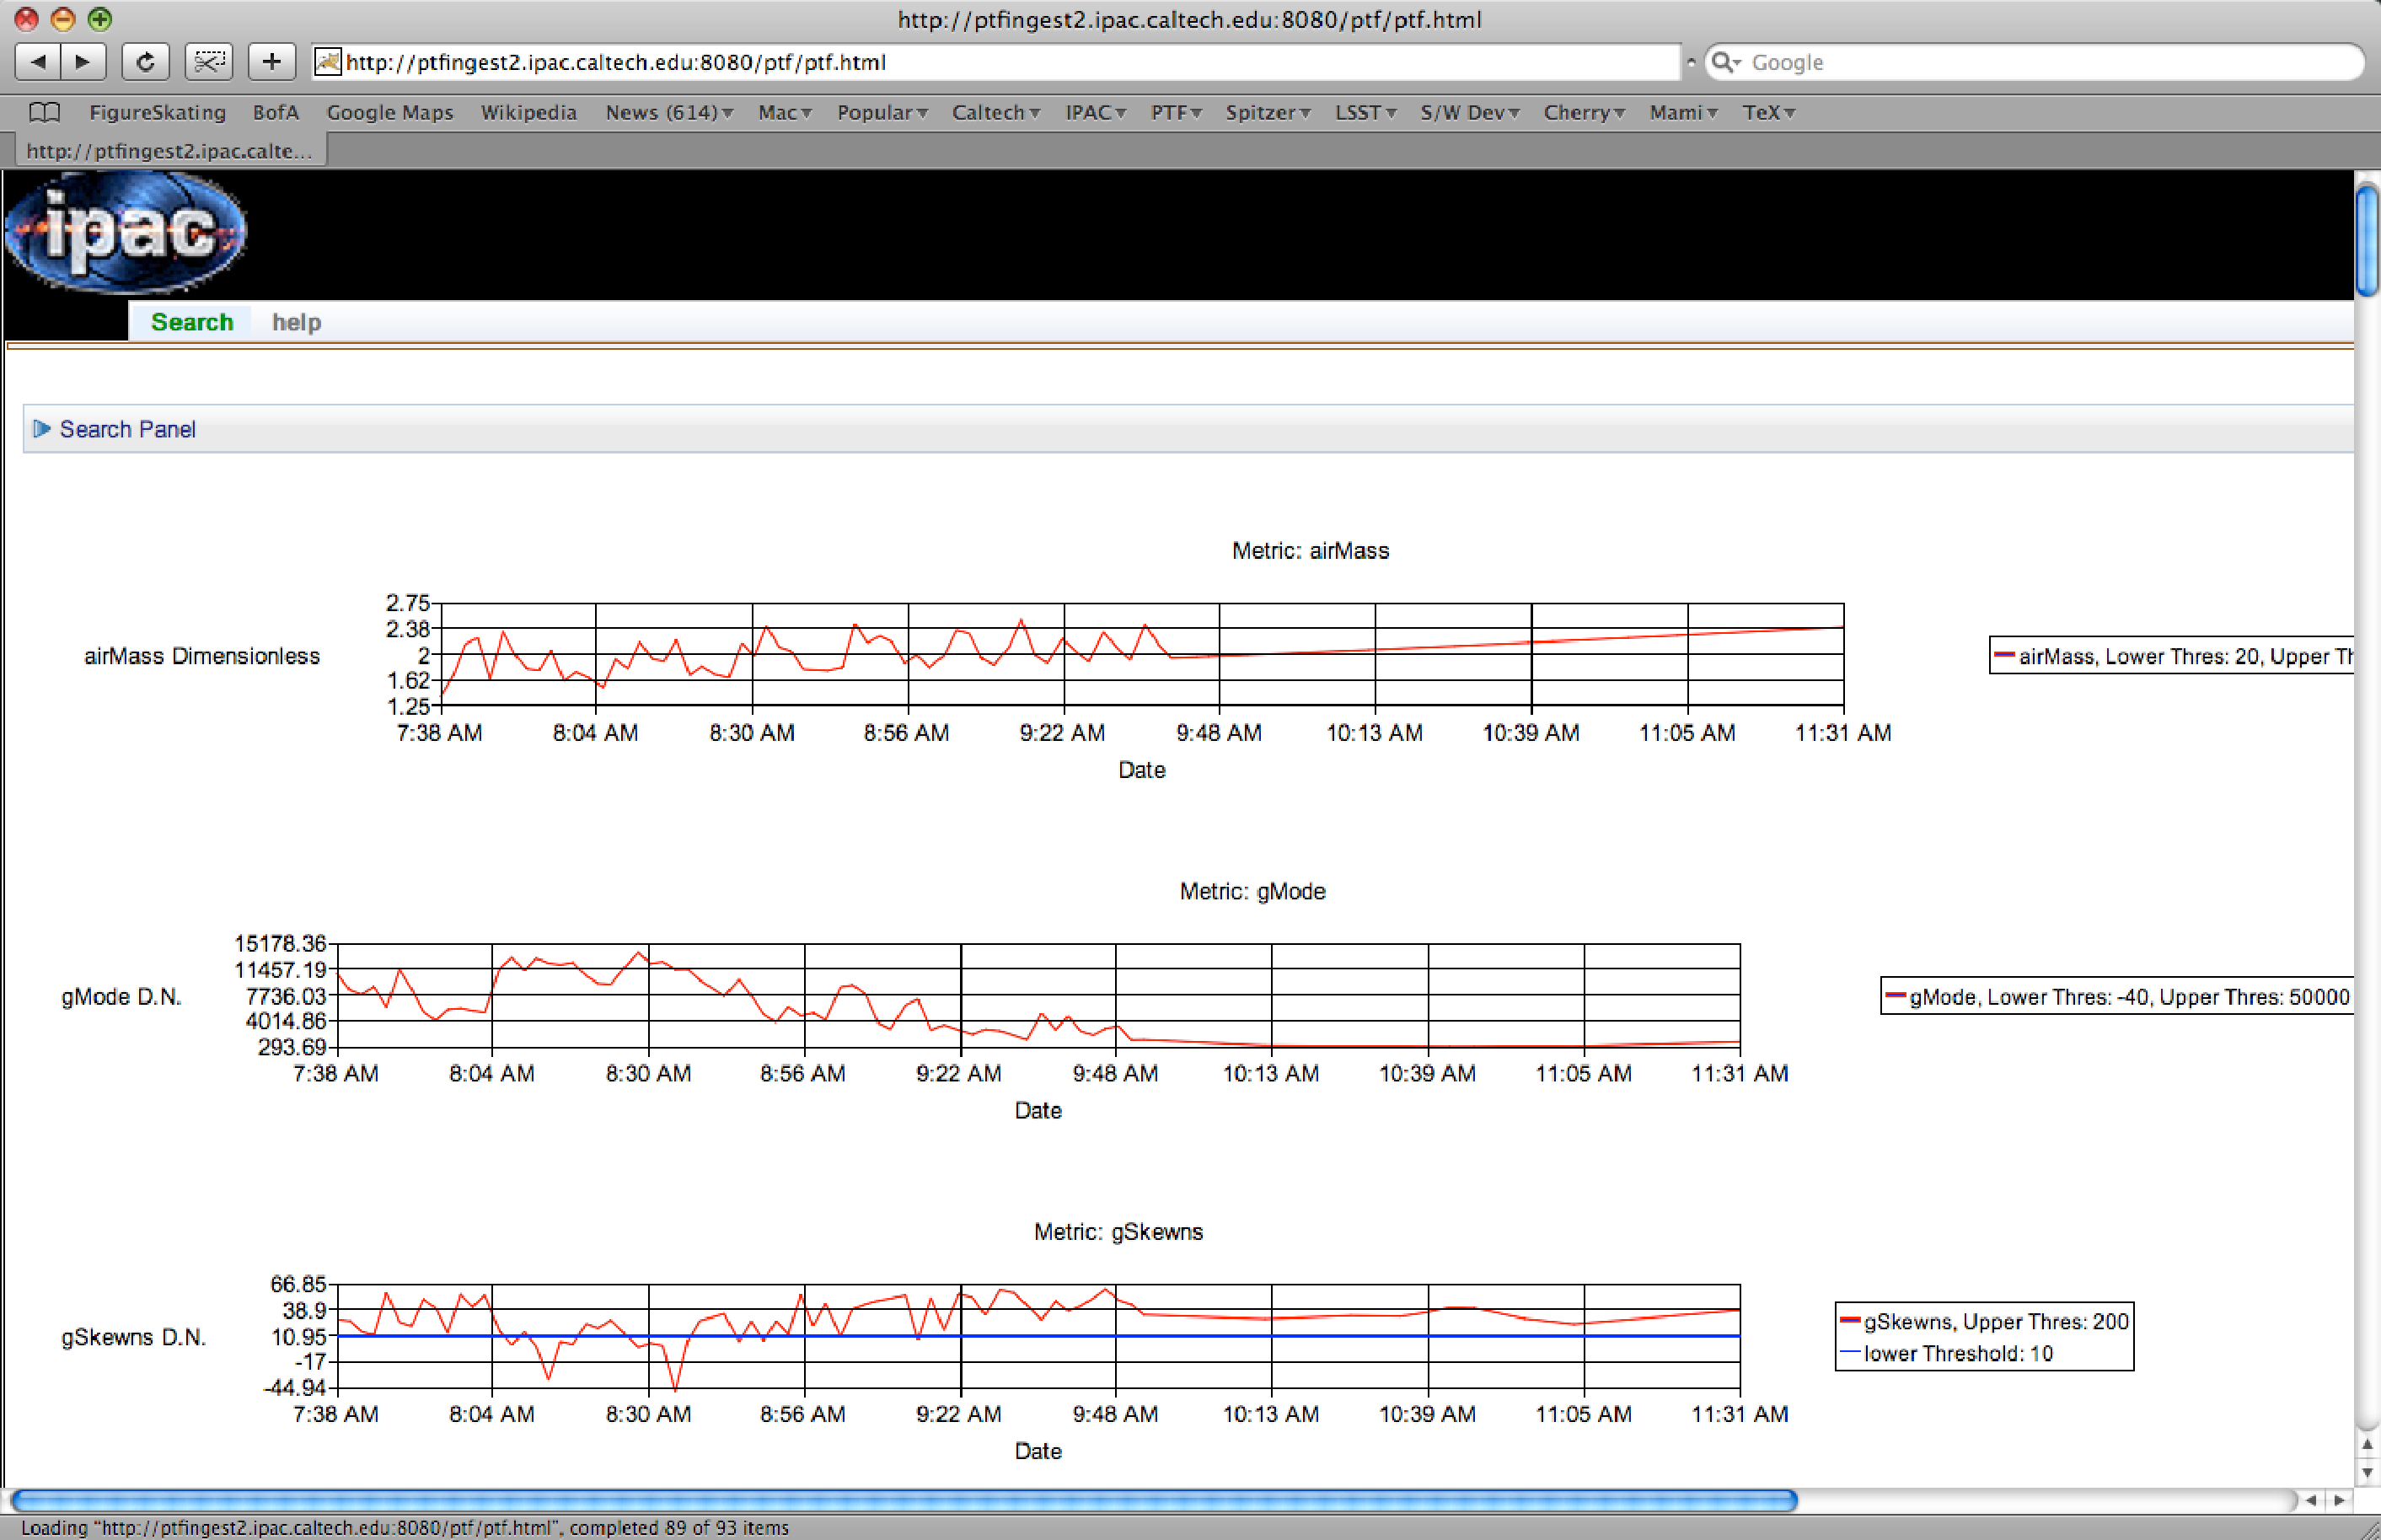
\includegraphics[width=\textwidth,bb=0 0 1356 877,clip]{images/PTFSDQSGUI2}
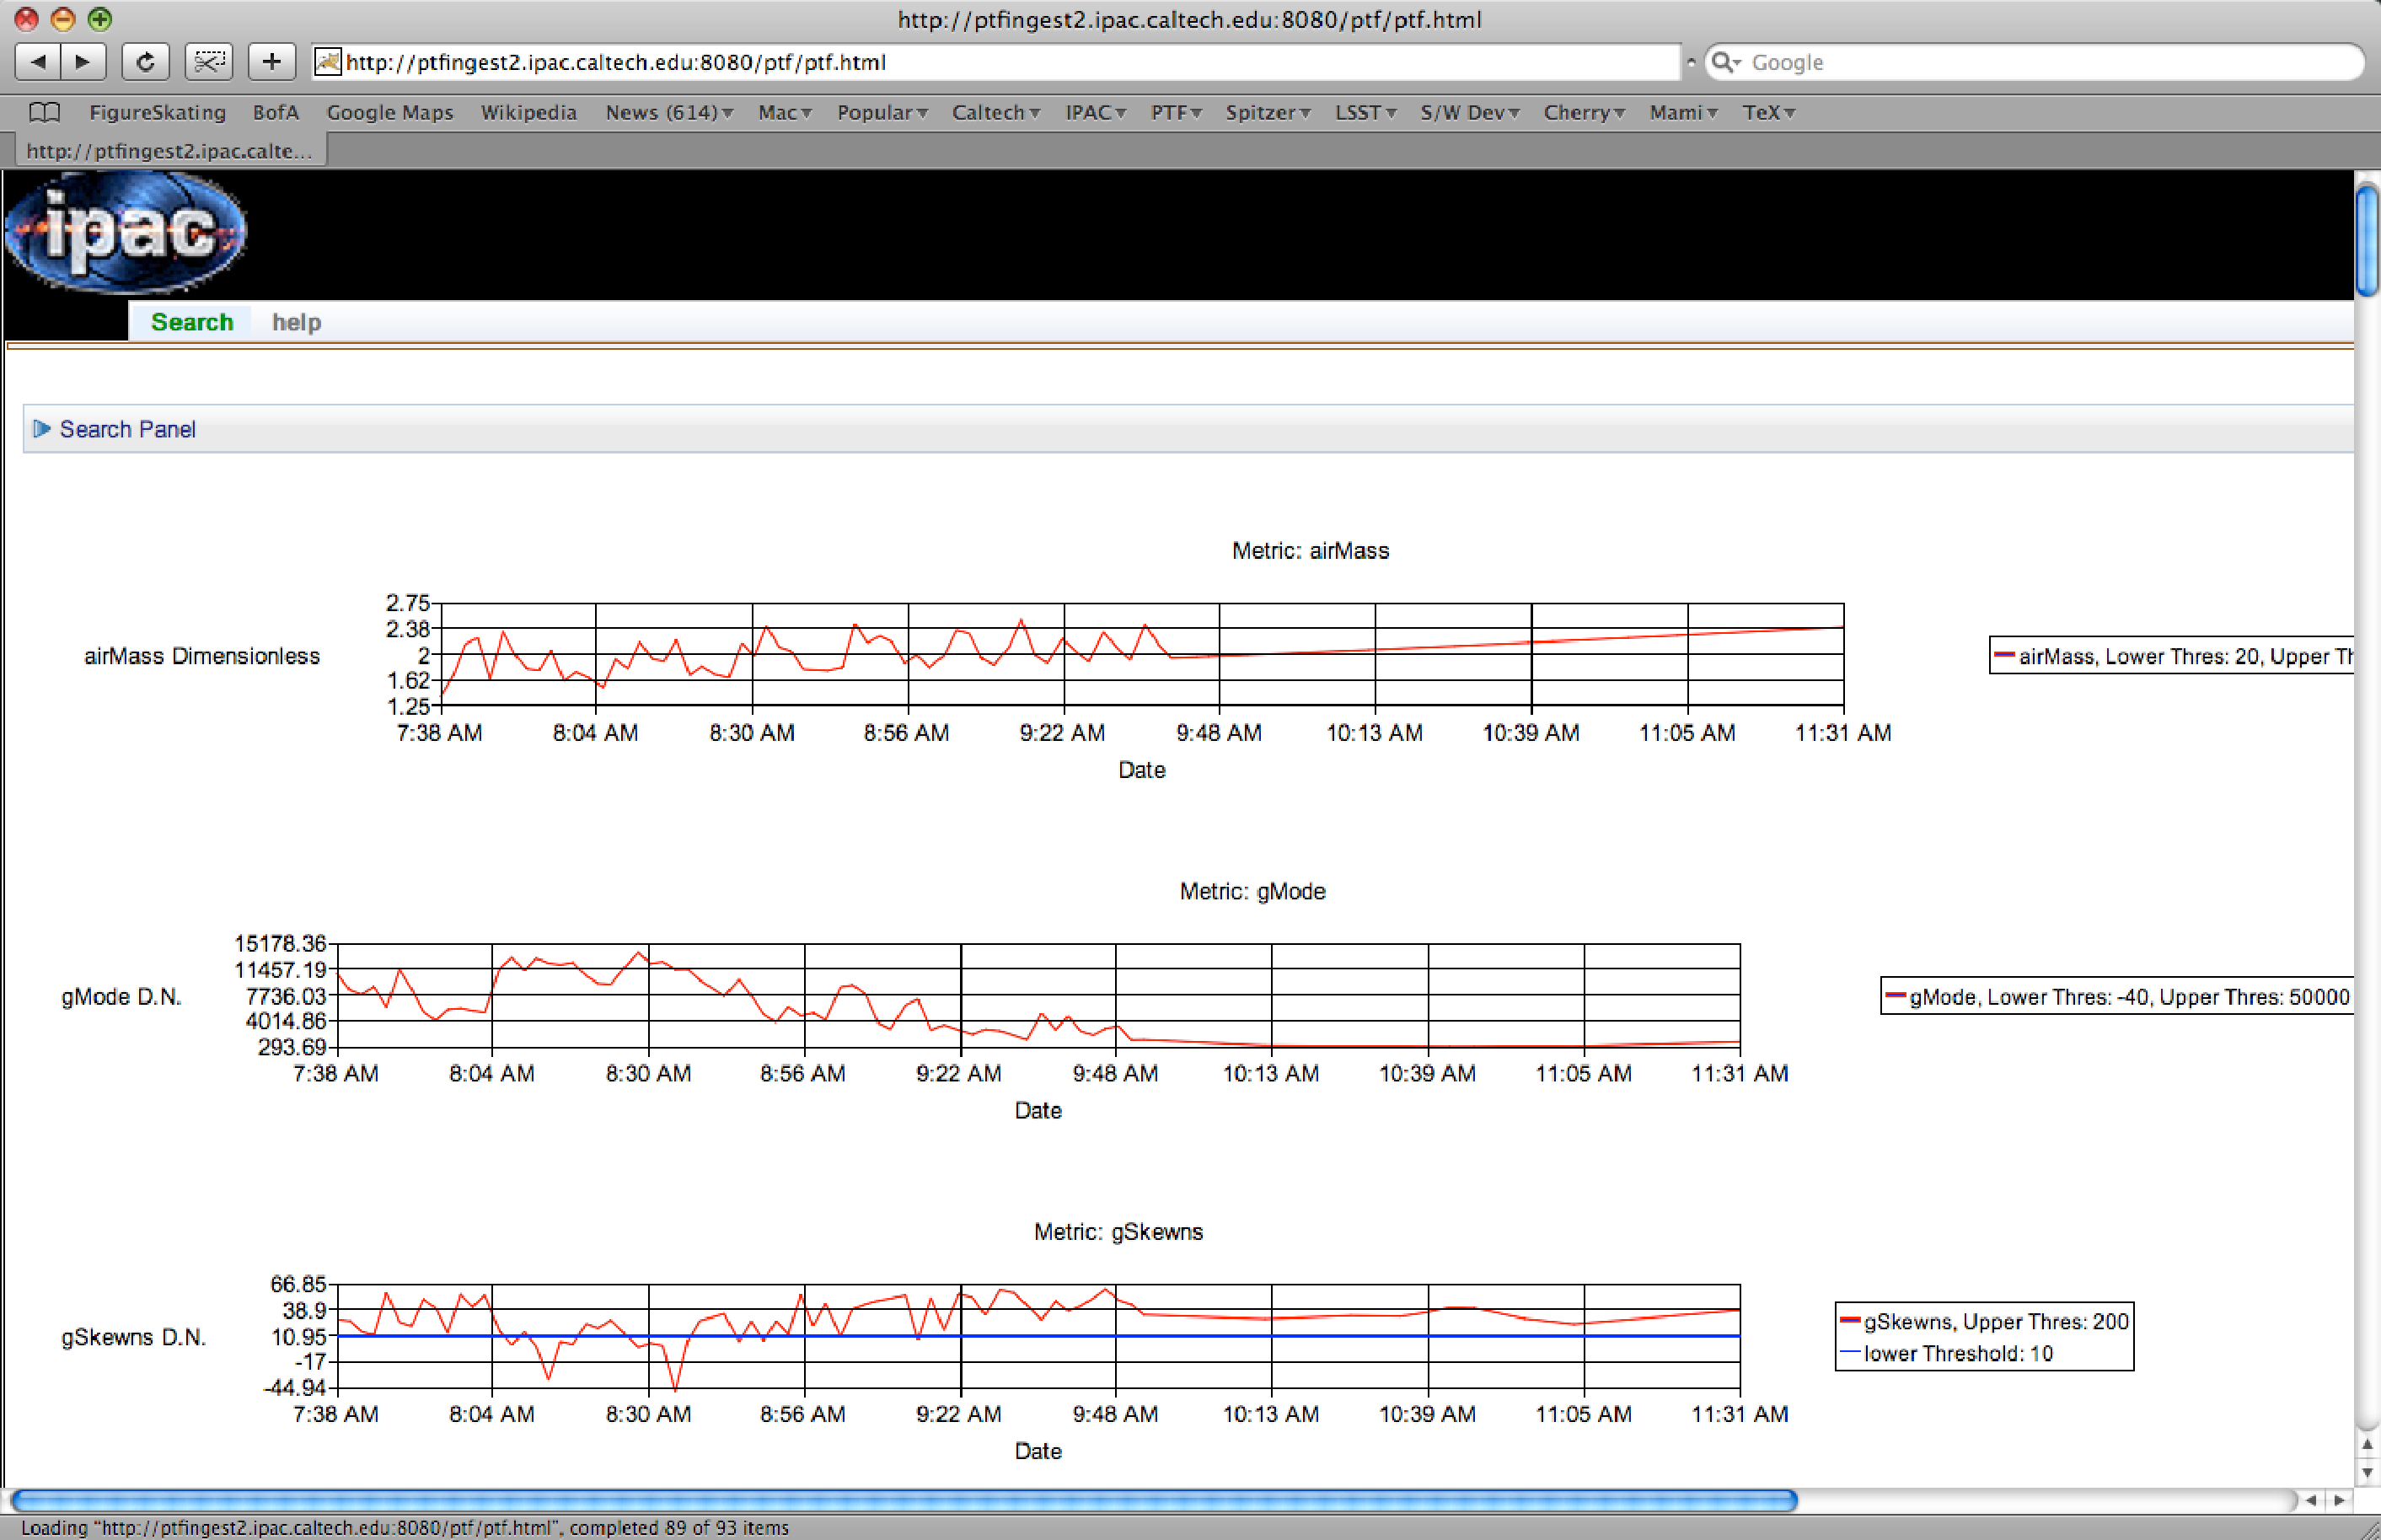
\includegraphics[width=5in]{images/PTFSDQSGUI2}
\caption{PTF SDQA GUI screen shot showing SDQA time-series plots from query of PTF database.} 
 \label{PTFSDQAGUI2}
\end{centering}
\end{figure}
